\section{Glasanje putem Interneta}

\begin{frame}{Glasanje putem Interneta}
        \begin{minipage}{0.6\textwidth}
            \begin{itemize}
                \item problemi sa glasovima države Florida, 
                \\predsednički izbori SAD, \\2000. godina
                \item akcije za poboljšanje pouzdanosti glasačkih sistema
                \item Estonija - 2005. godina
                \item Norveška - 2011. i 2013. godina
            \end{itemize}
        \end{minipage}
        \begin{minipage}{0.3\linewidth}
            \centering
            
            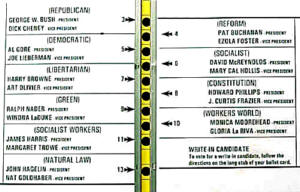
\includegraphics[scale = 1]{images/election.jpg}
        \end{minipage}
        
        \begin{itemize}
            \item danas je glasanje putem Interneta omogućeno u 14 zemalja \\(Kanada, Francuska, Švajcarska...)
        \end{itemize}
    \end{frame}
    
    
    \begin{frame}{Benefiti glasanja putem Interneta}
    		\begin{itemize}
    			\item daje ljudima priliku da glasaju iz svojh domova
			\item brže prebrojavanje glasova
			\item nema dvosmislenosti
			\item manji trošak
            \item eliminisanje rizika da neko manipuliše glasačkom kutijom
            \item obrazac za glasanje sa različitim ograničenjima
			\item veb forma dizajnirana više strana 
    		\end{itemize}
    \end{frame}
    
    
    \begin{frame}{Rizici glasanja putem Interneta}
    	\begin{itemize}
			\item daje prednost onima koji su u finansijski boljoj situaciji
			\item isti sistem vrši autentifikaciju glasača i beleži glasački listić
			\item povećava mogućnost za kupovinu i prodaju glasova.
			\item veb lokacija koja održava izbore očigledna je meta DDoS napada
			\item \textit{backdoor} Trojanac (eng. {\em backdoor Trojan})koji vreba na računaru glasača
			\item napadač može da prevari korisnika da misli da je povezan sa serverom za glasanje kada je u stvari povezan sa lažnim serverom za glasanje koji je kontrolisan od strane napadača	
		\end{itemize}
    \end{frame}